%-----------------------------------------------------------------------------%
\chapter{\babDua}
%-----------------------------------------------------------------------------%
Bab ini berisi tentang tinjauan pustaka yang terkait dengan penelitian. Bab ini akan menjelaskan mengenai ontologi, zotonic, dan \textit{software product line}.
%-----------------------------------------------------------------------------%
\section{Ontologi}
%-----------------------------------------------------------------------------%
	
Ontologi merupakan bagian yang paling mendasar dari web semantik. Ontologi
adalah sebuah deskripsi formal yang eksplisit tentang kelas (domain atau disebut juga sebagai \textit{concepts}), relasi, dan \textit{property} dari setiap domain, yang biasanya telah terdefinis secara baik \citep{hopkins_powell_2015}. Menurut \cite{ontologydevelopment}, pengembangan ontologi perlu dilakukan karena beberapa alasan berikut ini.

\begin{enumerate}
\item Berbagi pemahaman umum terkait struktur dari informasi diantara manusia ataupun \textit{software agents}.
\item Menggunakan kembali pengetahuan dari kelas.
\item Membuat asumsi terkait kelas tersampaikan secara eksplisit.
\item Memisahkan pengetahuan tentang kelas dari pengetahuan secara operasional.
\item Menganalisa pengetahuan tentang kelas.
\end{enumerate}

Berbagi pemahaman umum terkait struktur dari informasi merupakan satu dari beberapa tujuan utama pada pengembangan ontologi \citep{paper.gruber}. Dengan adanya pemahaman terkait struktur dari informasi yang diperoleh, sebuah \textit{software agents} dapat mengekstrak dan mengumpulkan informasi yang diperoleh dari berbagai layanan yang berbeda namun menggunakan dasar ontologi yang sama. Selain dapat memperoleh informasi, dengan menggunakan struktur ontologi yang cenderung sama maka sebuah ontologi dapat digunakan kembali untuk kasus yang cenderung sama atau mirip sehingga dapat melakukan penghematan dana maupun waktu.

Ontologi terdiri dari beberapa komponen yaitu kelas, atribut, relasi. Ketika membuat ontologi, kelas merupakan komponen yang harus dibuat pertama kali karena kelas merupakan komponen utama dari ontologi. Kelas atau disebut juga domain, merupakan kumpulan data pada ontologi yang memiliki sebuah nama yang deskriptif untuk menggambarkan data tersebut. Salah satu contoh dari kelas adalah sebagai berikut

\begin{figure}
	\centering
	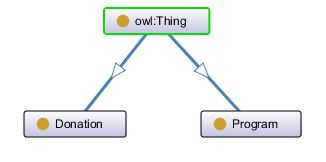
\includegraphics[width=0.7\textwidth]
	{pics/domain.jpg}
	\caption{Contoh Kelas pada Ontologi}
	\label{fig:class}
\end{figure}
\vspace{-0.3cm}

Pada \pic~\ref{fig:class}, Program dan \textit{Donation} merupakan salah satu contoh dari kelas (disebut sebagai \textit{thing} pada \textit{software} protege). Program merupakan kumpulan data mengenai kegiatan yang dilakukan sedangkan \textit{Donation} merupakan kumpulan data mengenai donasi terhadap suatu program. Kelas Program dan \textit{Donation} membutuhkan atribut yang akan menjelaskan tentang kelas tersebut sehingga perlu didefinisikan apa yang menjadi atribut dari kelas tersebut. Pada penelitian ini, penulis menggunakan ontologi yang sudah ada yaitu ontologi \textit{charity organization} dimana kelas Program memiliki atribut name dan total sedangkan kelas \textit{Donation} memiliki atribut \textit{amount}. Pada gambar \pic~\ref{fig:class}, belum terdapat keterhubungan diantara kelas Program dan \textit{Donation} sehingga perlu membuat komponen terakhir yaitu relasi. Setiap relasi harus dapat menggambarkan keterhubungan dari kelas yang ada. Pada ontologi \textit{charity organization} yang digunakan, kelas Program dan \textit{Donation} dihubungkan menggunakan relasi \textit{Channeled through} seperti gambar berikut

\begin{figure}
	\centering
	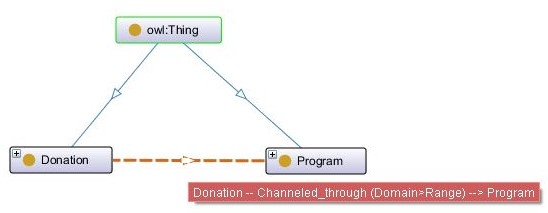
\includegraphics[width=0.9\textwidth]
	{pics/relationClass.jpg}
	\caption{Contoh Relasi pada Ontologi}
	\label{fig:relationClass}
\end{figure}
\vspace{-0.3cm}

Pada gambar \pic~\ref{fig:relationClass}, dapat dilihat bahwa kelas \textit{Donation} dan kelas Program dihubungkan oleh relasi \textit{Channeled through} yang berarti suatu donasi dapat disalurkan kepada suatu program. Relasi antar keduanya digambarkan sebagai sebuah edge pada graf ontologi. 

Selain memiliki tiga komponen yang telah disebutkan diatas, pada ontologi juga terdapat struktur hierarki yang dapat dimiliki oleh suatu kelas. Struktur hierariki ini menggambarkan tingkatan dari suatu kelas. Kelas yang memiliki tingkatan lebih tinggi biasanya merupakan kelas yang bersifat lebih umum dari kelas-kelas yang memiliki tingkatan lebih rendah dari dirinya. Sebagai contoh, kelas Hewan memiliki tingkatan yang lebih daripada kelas Mamalia dan juga kelas Reptil karena mamalia dan reptil merupakan bagian dari hewan. Hal ini dapat dilihat pada \pic~\ref{fig:subClass} dimana kelas \textit{EventualProgram} memiliki tingkatan yang lebih rendah dari kelas Program atau disebut dengan \textit{subclass}. Untuk kelas yang memiliki tingkatan yang lebih rendah dari kelas diatasnya, kelas tersebut akan mewarisi semua atribut atau properti yang terdapat pada kelas yang lebih tinggi dari dirinya. Sebagai contoh, kelas Program memiliki atribut \textit{name} dan total sehingga kelas \textit{ContinuousProgram, EventualProgram serta PeriodicProgram} akan memiliki atribut \textit{name} dan total juga.

\begin{figure}
	\centering
	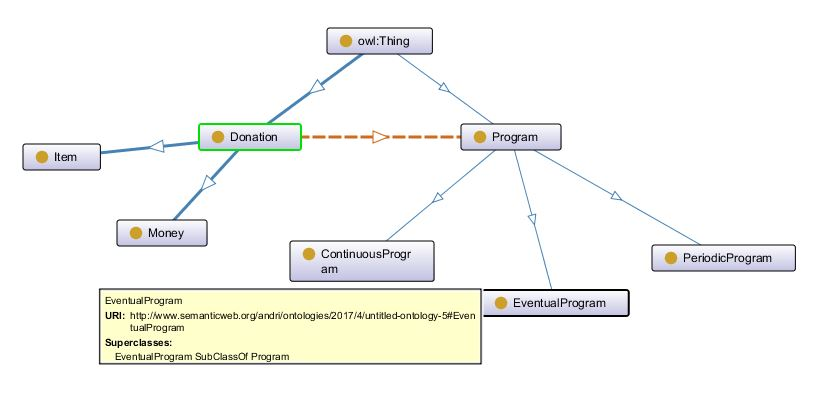
\includegraphics[width=1\textwidth]
	{pics/subClass.jpg}
	\caption{Contoh Struktur Hierarki}
	\label{fig:subClass}
\end{figure}
\vspace{-0.3cm}

Agar ontologi dapat dipahami oleh komputer, ontologi tersebut harus direpresentasikan dalam bentuk yang dapat dibaca oleh komputer salah satunya adalah OWL. \textit{Ontoloy Web Language} (OWL) merupakan versi RDFS yang memiliki kosa kata dan \textit{rules} yang lebih ketat sehingga OWL lebih mudah dipahami oleh komputer karena dapat lebih menggambarkan ontologi yang dibuat \citep{owl.overview}. Pada penelitian ini, digunakan setidaknya tiga elemen dari OWL yaitu \textit{class, datatype property} serta \textit{object property}. \textit{Class} akan menggambarkan kelas dari ontologi, \textit{datatype property} akan menggambarkan atribut dari kelas, serta \textit{object property} akan menggambarkan relasi antar suatu kelas dengan kelas lainnya.
%-----------------------------------------------------------------------------%
\section{Zotonic}
%-----------------------------------------------------------------------------%

Zotonic merupakan web yang bersifat \textit{open source}, \textit{real-time web framework}, dan sekaligus sebagai \textit{Content Management System} (CMS) yang dibangun menggunakan bahasa pemrograman erlang \citep{zotonic.overview}. Selain merupakan sebuah CMS dan \textit{framework}, Zotonic juga merupakan sebuah web server yang dapat menjalankan web langsung tanpa bantuan web server seperti Apache dan Nginx. Karena dibangun dengan bahasa pemrograman erlang, Zotonic sangat mengutamakan kecepatan.

Menurut Zotonic, kecepatan dari zotonic ini sendiri bisa mencapai 10x lebih cepat daripada CMS yang dibangun menggunakan bahasa pemrograman PHP. Hal ini berdasarkan perbandingan antara proses pembuatan halaman pada kebanyakan \textit{framework} PHP yang membutuhkan waktu 150-600 ms sedangkan pada Zotonic biasanya hanya membutuhkan waktu 10 ms atau kurang. Selain itu, Zotonic memiliki mekanisme untuk mencegah permintaan yang berbeda untuk melakukan hal yang sama pada waktu yang bersamaan. Ketika terdapat dua atau lebih permintaan datang untuk halaman yang sama, atau bagian dari halaman yang sama, maka zotonic akan melakukan pekerjaan sekali dan mengirimkan hasilnya ke semua permintaan yang masuk. Zotonic juga menyimpan data yang sering digunakan pada memori, sehingga dapat mencegah kueri yang banyak kepada database. Pada erlang, kode akan dimuat dan akan terus dimuat sampai ada perubahaan kode berikutnya sehingga hal ini dapat membuat zotonic lebih efisien dibandingkan PHP \citep{zotonic.speed}.

Zotonic juga menerapkan sistem modular. Zotonic dibuat dari lapisan kode yang umum dengan modul yang menyediakan fungsi utama lainnya. \textit{Template, actions, controllers, javascript, css, dispatch rules}, semuanya berasal dari modul. Modul dapat memperbanyak, mengubah atau bekerja sama dengan modul lainnya. Modul dapat mendefinisikan ulang \textit{template, javascript, css, actions} dan \textit{dispatch rules} dari modul lainnya.

Zotonic juga melakukan pemisahan antara model, tampilan, dan \textit{controller} atau biasa disebut MVC yang telah menjadi \textit{best practice} pada proses pembuatan web dalam waktu yang lama. Hal ini bagus untuk pemisahan tanggung jawab \citep{zotonic.mvc}. Hal ini akan memberikan kesempatan kepada \textit{programmer} dari program dan pengembang tampilan (\textit{front-ender}) untuk membuat HTML, CSS, dan lainnya sendiri berdasarkan kebutuhannya. Pengembang tampilan memiliki akses baca pada hampir semua informasi yang tersedia pada Zotonic. Pada \textit{template} dapat langsung memanggil kueri, mengambil \textit{properties} dari pages, melakukan pengecekan kunci konfigurasi, dan lainnya. Sehingga \textit{programmer} tidak butuh membuat \textit{controller} lainnya atau mengadopsi beberapa \textit{controller} untuk memberikan informasi ekstra kepada \textit{template}. Dan pengembang tampilan tidak perlu untuk menunggu \textit{programmer}. Hal ini berguna agar pengembang tampilan dapat secara langsung mengambil dan menampilkan data dari Zotonic pada \textit{template}.

Selain itu, tampilan pada zotonic dibangun menggunakan \textit{jQuery} dan CSS \textit{framework Bootstrap} yang merupakan salah satu CSS \textit{framework} yang sangat populer saat ini \citep{awwwards.css}. Selain penggunaan \textit{jQuery} dan \textit{Bootstrap}, Zotonic juga mengadopsi penggunaan ErlyDTL (\textit{Erlang implementation of the Django Template Language}). ErlyDTL digunakan agar pemuatan data dari basis data dapat dilakukan langsung dari \textit{template} yang ingin memuat data itu sendiri. Zotonic sendiri menambahkan beberapa fitur pada ErlyDTL yang diadopsi seperti untuk \textit{caching} dan \textit{template} hanya di\textit{compile} ke memori sehingga dapat mencegah masalah ketika logika internal dari \textit{template} berubah versi.

Selain itu, zotonic menawarkan fitur fleksibilitas pada model data. Hal ini karena zotonic memberikan kebebasan kepada penggunanya untuk melakukan penambahan atau pengurangan terhadap model data. Model data pada Zotonic sendiri merupakan bentuk implementasi dari web semantik. Model datanya memiliki dua konsep utama yaitu \textit{resource} dan \textit{edge} \citep{zotonic.model}. \textit{Resource} pada Zotonic biasanya disebut sebagai \textit{pages} pada halaman admin karena semua \textit{resource} yang dihasilkan pada aplikasi akan ditampilkan sebagai sebuah \textit{pages}. \textit{Resources} memiliki bagian utama yaitu mereka memiliki \textit{properties} seperti judul, ringkasan, dan isi bodi serta mereka milik dari sebuah \textit{category}.

\begin{figure}
	\centering
	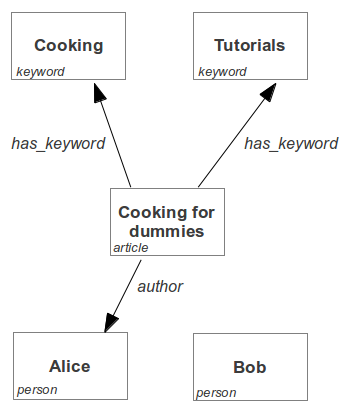
\includegraphics[width=0.6\textwidth]
	{pics/dataModel.png}
	\caption{Contoh Data Model}
	\label{fig:dataModel}
\end{figure}
\vspace{-1cm}
\begin{center}
{\small Sumber gambar: \citep{zotonic.model}}
\end{center}

Pada \pic~\ref{fig:dataModel}, blok persegi menggambarkan \textit{resource} dan panah menggambarkan \textit{edge}. Alice adalah sebuah \textit{resource} yang berkategori \textit{person}. Begitu juga halnya dengan Bob yang merupakan \textit{resource} dengan kategori \textit{person}. Hal ini menunjukkan bahwa pada Zotonic, suatu kategori dapat memiliki banyak \textit{instance} yang berupa \textit{resource}. \textit{Cooking} dan \textit{Tutorials} sama-sama merupakan \textit{resources} yang berkategori \textit{keyword} sedangan \textit{Cooking For Dummies} merupakan \textit{resource} yang berkategori \textit{article}. \textit{has\_keyword} merupakan \textit{edge} yang menunjukan hubungan antara suatu \textit{resource} dengan \textit{resource} lainnya. Hal ini dapat dilihat bahwa \textit{resource cooking for dummies} memiliki \textit{keyword} yaitu \textit{cooking} dan \textit{tutorials}. Dengan kata lain, kategori \textit{article} memiliki hubungan dengan kategori \textit{keyword} yaitu \textit{article} mempunyai \textit{keyword}. Ini sama dengan relasi yang menghubungkan suatu \textit{class} dengan \textit{class} lainnya pada ontologi. Dengan model data yang seperti ini, zotonic merupakan salah satu CMS yang menerapkan implementasi dari web semantik.
%-----------------------------------------------------------------------------%
\section{\textit{Software Product Line}}
%-----------------------------------------------------------------------------%
	\todo{Jelasin SPL itu apa.}
